\begin{abstract}
Three-dimensional layer codes combine local stabilizer checks with high storage
density, but computation also requires local access to their logical operators.
We give an explicit local realization of the Williamson--Baspin layer code for
any CSS input whose checks have weight at least two, and prove that it encodes
exactly the input logical qubits, that every pure-$X$ logical class has a
representative on a single lattice layer, at every height of the block, and
that every pure-$Z$ class has one in a single transverse plane, at every
position.  A running (prefix) parity along each check sheet gives these
representatives.  The slabs support logical Pauli measurements by
nearest-neighbor three-dimensional grid gauging.  A constant number of
ancillas per grid edge preserves the full code distance, whereas a measurement
layer of bounded thickness provably cannot: a thin interface contains a wall
of few edges that a few faults can cross.  Circuit-level simulations on
explicit layer-code blocks confirm both statements; as the blocks grow,
failures through the grid fall and failures through a one-row interface rise.
We then observe these distance mechanisms on IQM and IBM superconducting
processors, with three-qubit blocks and \hwTotalShots~million samples.
Widening the interface from one edge to two lowers the error of a joint
measurement \hwIQMfold-fold on IQM (from \hwIQMwOne\% to \hwIQMwTwo\%, with no
failure in \hwIQMwThreeKept{} samples at three edges) and
\hwIBMfoldOneTwo-fold on IBM, and two parallel ancillas on one edge lower it
\hwMultFold-fold on IQM.  Repeated rounds protect the reported bit as a calibrated
model predicts when every round uses fresh ancillas.  When ancillas are
measured and reset instead, errors that survive the reset, most likely
leakage, leave the three-round error \hwRndIBMModelRatio~times above the
calibrated Pauli model, a failure mode outside local-stochastic noise.
Lifting the input distance through the slabs shows that the realization has
the optimal distance $\Theta(N^2)$ for good inputs.  Combining the
measurements with encoded resource transfer, distillation, and a local
detector schedule gives a universal fault-tolerant architecture under
local-stochastic Pauli noise.  At fixed noise below an existential threshold,
a depth-$T$ circuit on $W$ logical sites in a bounded-aspect box uses
$O(Wf+f^{3/2})$ physical qubits and $O(Tf^{3/2}\Psi)\subseteq O(Tf^{5.41})$
depth, where $f=\Theta(\log(WT/\varepsilon))$ and $\Psi=O(f^{\log_215})$ is
the distillation depth factor; a concrete estimate places the storage
advantage at distances of order a thousand.  We also derive a fragmentation
correction for general regions and port-packing bounds saturated by balanced
layer codes.
\end{abstract}
\maketitle
\raggedbottom

\section{Introduction}
Quantum error-correcting codes must protect stored information and make that
information accessible to computation. These demands can pull in different
directions: a code with favorable storage parameters may still require costly
logical measurements or physical connections that are difficult to realize.
Three-dimensional layer codes provide a natural setting in which to address
this problem. The construction of Williamson and Baspin embeds a CSS code into
a local network of surface-code sheets and defects \cite{WilliamsonBaspinLayerCodes}.
For balanced good low-density parity-check inputs of length $N$, the resulting
blocks have
\begin{equation}
 n=\Theta(N^3),\qquad K=\Theta(N),\qquad d=\Theta(N^2),
 \label{eq:parameters}
\end{equation}
with bounded-weight, geometrically local stabilizers. Here $n$ is the physical
block size, $K$ its number of logical qubits, and $d$ its distance.

The central result of this work is a geometric interface for processing that
stored information.  We give an explicit lattice realization of the layer code
with complete check matrices, and show that every pure-$X$ logical class has a
representative on a single layer of the lattice and every pure-$Z$ class one in
a single transverse plane.  The layer can be placed at any height, and the
plane at any position, independently of $N$ and of the chosen logical
operator.  This converts an algebraic choice of logical Pauli into a
spatially localized measurement port.

We use this interface to construct universal fault-tolerant computation on the
native three-dimensional nearest-neighbor lattice.  The argument has three
steps. A prefix-parity construction first produces the slab representatives.
Relative expansion of a cubic grid then gives a local gauging measurement with
distance $\Omega(d)$. Finally, repeated extraction, padded composition, and
encoded resource transfer give a complete circuit under local-stochastic Pauli
noise. Figure~\ref{fig:overview} summarizes the architecture.

\begin{figure*}[t]
\centering
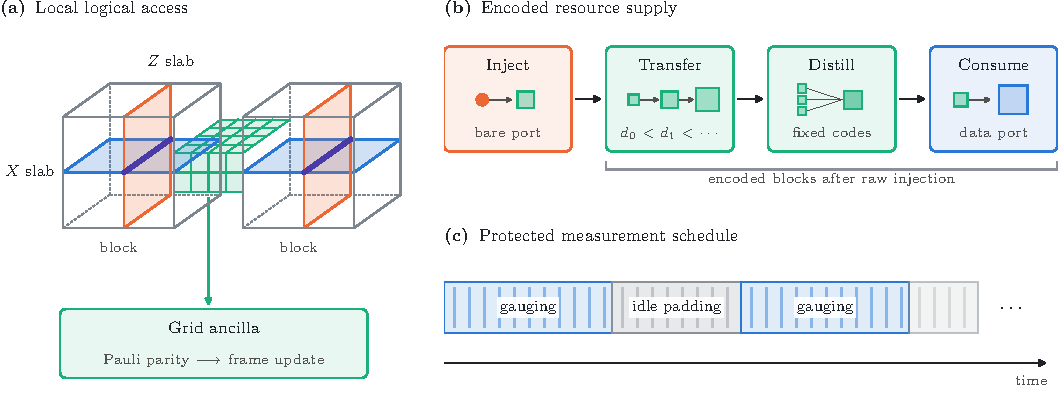
\includegraphics[width=\textwidth]{revision_architecture.pdf}
\caption{Geometry-preserving processing. (a) A layer-code block exposes
transverse slab ports for pure-$X$ and pure-$Z$ logical operators. A local grid
ancilla measures the selected Pauli; neighboring blocks use the same interface
for joint measurements. (b) A raw resource is injected into an encoded block,
transferred through blocks of increasing distance, distilled, and consumed by
the data path. (c) Repeated extraction and idle padding connect successive
active measurements. All drawings are schematic; the encoded blocks and grid
ancillas occupy three-dimensional regions.}
\label{fig:overview}
\end{figure*}

Logical measurement by gauging, surgery, and homological constructions has
become a general route to processing quantum LDPC codes
\cite{WilliamsonYoderGauging,CowtanParallelSurgery,YuanParsimonious2026,IdeHomological,BerentLiftedSurgery}.
Adapters, extractors, and universal architectures address complementary
questions of connectivity, parallelism, and resource overhead
\cite{SwaroopAdapters,HeExtractors,ZhangGoodQLDPC,MalcolmEfficientQLDPC}.
Here the organizing constraint is three-dimensional Euclidean locality:
logical access, resource delivery, and syndrome extraction use the same
nearest-neighbor geometry. The layer-code slab theorem supplies the missing
connection between the memory construction and these processing primitives.

Locality also fixes the achievable overhead. In three dimensions a local
stabilizer code obeys $Kd=O(n)$ \cite{BPT}, so $\Theta(d)$ physical qubits
per logical qubit is the best possible storage cost, and layer codes attain
it. Surface-code patches processed by lattice surgery use $\Theta(d^2)$
qubits per logical qubit \cite{HorsmanLatticeSurgery,LitinskiSurgery}, and
three-dimensional surface and color codes trade larger volume for
transversal gates \cite{VasmerBrowne}. Local simulations of LDPC codes
\cite{PattisonHierarchical}, local fault-tolerance constructions
\cite{ChoeKoenigLocal}, wire codes \cite{BaspinWire}, and planar logical
measurements \cite{YangPlanar} address related geometric questions, while
constant-overhead schemes
\cite{GottesmanFTThreshold,KovalevPryadko,FawziGrospellierLeverrier} and LDPC
magic-state injection \cite{ZhangInjectionIndependence,LiuInSituInjection}
rely on nonlocal connectivity. The architecture below keeps the
$\Theta(d)$-per-logical storage cost during computation, up to the cost of
one encoded cell.

The distance mechanisms behind the gauging measurements already act in circuits
small enough for present processors, so we also observe them on hardware
(Sec.~\ref{sec:hardware-main} and Fig.~\ref{fig:hardware}).  On IQM and IBM
superconducting processors, with three-qubit blocks in place of layer-code
blocks, a joint measurement through an interface of one edge fails
\hwIQMfold~times more often than through an interface of two edges on IQM, and
\hwIBMfoldOneTwo~times more often on IBM, as the cut obstruction predicts; two
parallel ancillas on the single edge lower the error
\hwMultFold-fold on IQM; and repeated rounds protect the reported bit.  The runs also
expose a limit of the noise model.  On IBM, ancilla errors that survive a
reset, most likely leakage, repeat the same wrong outcome in every round and
leave the three-round error \hwRndIBMModelRatio~times above a calibrated Pauli
model.  Such correlated faults lie outside the local-stochastic model of our
theorem, so an implementation of its schedule would need leakage reduction.

The main text develops the construction and the resource accounting, with
proof sketches at each step, and reports a complete circuit-level simulation
of one two-block logical measurement on explicit layer-code blocks and the
hardware demonstrations of its distance mechanisms. Complete proofs, cell coordinates, detector
templates, and numerical controls appear in the Supplemental Material
\cite{Supplemental}. We also show that the same slab mobility saturates a
logical-port packing bound and restricts shallow code-preserving unitaries.
These structural consequences are independent of the fault-tolerance proof.

\section{Logical operators in constant-thickness slabs}
\label{sec:slabs}
\subsection{The layer code as glued sheets}
A layer code is assembled from surface-code sheets
\cite{WilliamsonBaspinLayerCodes}.  Each qubit $q$ of the input CSS code
becomes a \emph{data sheet}, the plane $y=Y_q$; each input $Z$ check becomes
a $Z$-check sheet, a plane $x=\mathrm{const}$; and each input $X$ check
becomes an $X$-check sheet, a plane $z=\mathrm{const}$.  Every sheet is an
ordinary surface code on a rectangle of the cubic lattice, so it carries
string operators.  A string of $X$ operators that runs from one side of a
sheet to the other commutes with all checks of that sheet; a string that
stops inside the sheet leaves a violated check, a \emph{defect}, at its end.
A $Z$-check sheet meets the data sheets of the qubits in its check along
vertical lines, the \emph{junctions}.  Ordered along the check, these are its
first, middle, and last junctions.  The $X$-check sheets are attached in the
same way, with $X$ and $Z$ exchanged.

A junction is a rule that says which strings may end on the line without
leaving a defect.  For the $X$ strings used below only their presence
matters.  At a first or last junction the $Z$-check sheet ends on the data
sheet, and a string may pass from one sheet to the other: the check-sheet
string is present exactly when the data string is.  At a middle junction
three strings meet the line: the data string, which crosses it, and the
check-sheet strings on its two sides.  They leave no defect exactly when an
even number of the three is present.  Writing $1$ for a present string, and
listing the check-sheet strings first (left, then right) and the data string
last,
\begin{align}
 H_{\rm end}&=\begin{bmatrix}1&1\end{bmatrix}, &
 \ker H_{\rm end}&=\{00,11\},\nonumber\\
 H_{\rm mid}&=\begin{bmatrix}1&1&1\end{bmatrix}, &
 \ker H_{\rm mid}&=\{000,110,101,011\}.
 \label{eq:boundary}
\end{align}
Williamson and Baspin state these rules as sets of condensed anyons, that is,
as the combinations of string endpoints that disappear at the line;
Eq.~\eqref{eq:boundary} is the same information written for $X$ strings
(Supplemental Sec.~\ref{SM-app:source-trace}).  The word $110$ is the
important one.  It lets a string on the check sheet pass a data sheet without
any string on that data sheet.  If a middle junction allowed only $000$ and
$111$, every check-sheet string would drag a string onto each data sheet it
passes, and a general logical operator could not be built; such a lattice in
fact fails to encode the input qubits (Supplemental
Sec.~\ref{SM-sec:certificate}).

\subsection{An explicit lattice for the junctions}
We build every junction on the lattice (Supplemental
Sec.~\ref{SM-sec:explicit-realization}).  Sheets own distinct qubits, and
each junction rule adds one qubit of one sheet to one check of the other.  At
a middle junction the $Z$-check-sheet face beside the line gains the data
sheet's edge on the line.  That face then contains three qubits of interest:
the check-sheet edge on the line, where the string from one side ends; the
next check-sheet edge, where the string on the other side begins; and the
added data edge.  Its check is therefore exactly the middle rule of
Eq.~\eqref{eq:boundary}.  The data stars on the line gain the check sheet's
edges on the same side, which keeps them commuting with the modified faces.
At a first or last junction the check sheet ends on the data line and shares
its edges, which gives the two-bit rule.

One more repair is needed.  An $X$-check sheet and a $Z$-check sheet cross
along a line, and there the junction additions of the two sheets make a few
stars and faces anticommute, once for each data qubit shared by the two input
checks.  A row of one-qubit additions along the crossing line, which we call
a \emph{wall}, removes these conflicts.  It exists exactly when the shared
number is even, which is the commutation of the two input checks.  The slab
operators below never use wall qubits, so the walls play no further role.
Every check lies within unit distance of one lattice vertex and has weight at
most six.  Supplemental Fig.~\ref{SM-fig:junction-geometry} draws one junction
of each kind and a wall.  The junctions have the condensed anyons of
Ref.~\cite{WilliamsonBaspinLayerCodes}; we do not claim that the lattice is
identical to the drawings there, and all results below are proved for this
explicit lattice, whose complete check matrices the source package generates.

\subsection{Slab representatives}

\begin{theorem}[Uniform slab representatives]
\label{thm:slabs}
For every input CSS code with checks of weight at least two, the explicit
realization encodes exactly $K$ logical qubits.  Every pure-$X$ logical class has a representative supported
on the single layer of $z$-edges spanning $[z_0,z_0+1]$, for every height
$z_0$ of the block, and every pure-$Z$ class has a representative in the plane
$x=x_0$, for every $x_0$.  The heights and planes are chosen independently of
the logical classes.
\end{theorem}

The operator is built at one fixed height $z_0$, one input check at a time.
Choose a pure-$X$ logical $x\in\ker H_Z$ of the input code, and put an $X$
string at height $z_0$ on the data sheet of every qubit with $x_q=1$.  Each
such string crosses the junction of every $Z$-check sheet attached to its
data sheet, and on its own would leave a defect there.  Along one $Z$-check
sheet the selected junctions must therefore be joined, in pairs, by strings on
the check sheet at the same height; we call these check-sheet strings the
\emph{backbone}.  Pairing is possible because $x$ commutes with the input
check, so the check contains an even number of selected qubits.  Walk along
the check from its first qubit and switch the backbone on or off at every
selected junction.  With ordered incidences $x_1,\ldots,x_k$, the backbone
after the $i$th junction is present exactly when an odd number of selected
qubits lies behind it, a running count that we call the \emph{prefix parity},
\begin{equation}
 p_0=0,\qquad p_i=\sum_{h=1}^{i}x_h,\qquad p_k=0,
 \label{eq:prefix}
\end{equation}
where $p_k=0$ is the commutation $\sum_ix_i=0$ over $\mathbb F_2$.  At every
middle junction $p_{i-1}+p_i+x_i=0$, so none or two of the three strings are
present, as Eq.~\eqref{eq:boundary} requires; at the ends $p_1=x_1$ and
$p_{k-1}=x_k$.  No defect remains anywhere (Fig.~\ref{fig:slab-prefix}).
Every piece lies in the same layer of vertical edges, so the operator is one
lattice layer thick, whatever the block size and whichever logical is
chosen.  Building it at another height gives another representative of the
same class.  In the explicit realization the check is exact and local: every
stabilizer meets the operator in one of the forms $x_1+p_1$,
$p_{i-1}+p_i+x_i$, $p_{k-1}+x_k$ of a single incidence, or not at all.

\begin{figure*}[t]
\centering
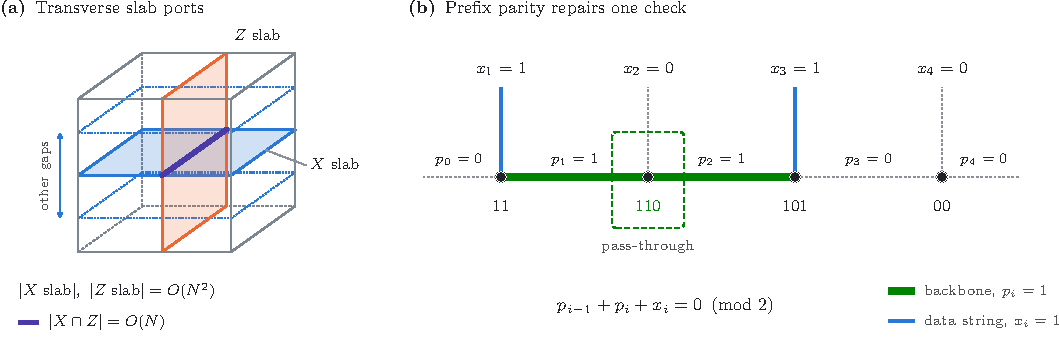
\includegraphics[width=\textwidth]{revision_slab_prefix.pdf}
\caption{Slab mobility and its local mechanism. (a) Complete $X$ and $Z$ ports
occupy transverse single-layer slabs. Each slab contains $O(N^2)$
qubits, and their intersection contains $O(N)$ qubits. Translating to another
height (or plane) gives another representative of the same logical class.
(b) For the even incidence word $(1,0,1,0)$, the running parity is
$(0,1,1,0,0)$. The highlighted middle cell uses $110$: the backbone remains
occupied although the data incidence is absent. Endpoint cells use the
two-bit relation in Eq.~\eqref{eq:boundary}.}
\label{fig:slab-prefix}
\end{figure*}

The pure-$Z$ operators are built in the same way in a vertical plane
$x=x_0$, with backbones on the $X$-check sheets.  An $X$ slab operator and a
$Z$ slab operator share only one data edge for each input qubit selected by
both, so they anticommute exactly when the two input logicals do.  This gives
$K$ independent logical qubits.  A count shows that there are no others.  On
its own, each data sheet would encode one qubit and each check sheet would
remove one; the junctions and walls add neither qubits nor checks; and every
redundancy among the lattice checks comes from a redundancy among the input
checks.  In formulas, each data sheet contributes $+1$ and each check sheet
$-1$ to $n-\#X-\#Z$, and the relations among the lattice checks inject into
those among the input checks.  Hence the realization encodes at most, and
therefore exactly, $K$ qubits, and the slab operators represent every
pure-type class.  A certificate on complete codes
with up to $10{,}936$ qubits, including the linear forms above, exhaustive
negative controls, and the single-chart comparison, checks each step
(Supplemental Sec.~\ref{SM-sec:certificate}). The proofs are Supplemental
Proposition~\ref{SM-prop:explicit-k} and Theorem~\ref{SM-thm:slab-resolved}.

Williamson and Baspin already obtain the layer-code logical operators by
quasi-concatenating input logicals \cite{WilliamsonBaspinLayerCodes}.  The
new ingredients are an explicit realization in which this construction can
be verified check by check, a single-layer thickness independent of the block
size and of the chosen logical, and its uniformity over every height, which
supplies the disjoint ports used below.

The same ports give the distance, by a simple idea: a logical operator must
be visible in every plane that contains a complete port of the other type.
Let $O$ be a nontrivial $X$ logical.  It anticommutes with some $Z$ logical,
and that $Z$ logical has a slab representative in each of the $L_x+1$
disjoint planes $x=x_0$, so $O$ must place qubits in every one of these
planes.  To count them, cut the $Z$ slabs of one plane into their pieces: a
vertical data column for each input qubit, and the backbone segments.
Record, for each piece, whether $O$ meets it an odd number of times.  Read a
data piece as its input qubit, and a backbone piece as the qubits of its
input $X$ check that lie behind it, the first $t$ of them for the $t$th
segment.  The records then spell out a nontrivial $X$ logical of the input
code, which has at least $d_X^{\rm in}$ entries.  The first $t$ qubits of a
check may be exchanged for the remaining ones, because the whole check is a
stabilizer of the input code, so a backbone piece stands for at most
$\eta_X=\max\{1,\lfloor w_X/2\rfloor\}$ qubits, where $w_X$ is the largest
input $X$-check weight.  Each piece met an odd number of times holds at least
one qubit of $O$, so each plane contains at least
$\lceil d_X^{\rm in}/\eta_X\rceil$ qubits of $O$, and
\begin{equation}
 d_X\ge(L_x+1)\left\lceil\frac{d_X^{\rm in}}{\eta_X}\right\rceil,
 \label{eq:distance}
\end{equation}
dually for $Z$.  For balanced good inputs the realization therefore has
$n=\Theta(N^3)$, $K=\Theta(N)$, and $d=\Theta(N^2)$, the parameters of
Eq.~\eqref{eq:parameters} (Supplemental
Theorem~\ref{SM-thm:explicit-distance}).  For the $[[4,2,2]]$ and $[[6,4,2]]$
inputs the bound equals the exact distance in every computed instance.

For balanced inputs the block has $\Theta(N)$ heights and $\Theta(N)$
transverse positions, so there are
\begin{equation}
 r_X=\Theta(N),\qquad r_Z=\Theta(N)
 \label{eq:mobility}
\end{equation}
pairwise-disjoint slab regions within each orientation. Each region is a
complete port for its logical polarization. This repeated access will also
give the structural bounds in Sec.~\ref{sec:structure}.

\section{Local gauging and universal logical operations}
\label{sec:measurements}
\subsection{Why a three-dimensional grid preserves distance}
Gauging measures a logical operator by measuring many small checks whose
product is that operator \cite{WilliamsonYoderGauging}.  Let
$\overline P=X(D)$ be the selected logical representative.  Attach each data
qubit of $D$ to its own vertex of a connected grid $G=(V,E)$, call these
vertices the \emph{ports} $U$, and place an ancilla qubit on every edge.  The
new check at a vertex, its \emph{vertex star}, is $X$ on the edges at that
vertex and on the attached data qubit, if any.  Every edge belongs to two
vertex stars, so the product of all vertex stars is $\overline P$, and the
product of their measured outcomes is the logical outcome; yet each
measurement involves only a few neighboring qubits.  The grid also carries
$Z$ checks around its unit squares, and every original $Z$ check that meets
$D$ is extended along short grid paths joining its ports, so that it commutes
with the stars.  Preparing the edge qubits in $|0\rangle$, measuring the new
checks, and finally reading the edges in $Z$ returns the data to its original
code with an updated Pauli frame.  The $X/Z$-exchanged construction measures
pure-$Z$ logicals.

The danger is that the added qubits create new, shorter logical operators.
The quantity that controls this is the expansion of the grid relative to its
ports,
\begin{equation}
 \beta(G,U)=\min_{S\subseteq V}
 \frac{|\delta S|}{\min\{|S\cap U|,|U\setminus S|\}},
 \label{eq:beta}
\end{equation}
where $\delta S$ is the set of edges leaving $S$ and only positive
denominators are included.  We call $\delta S$ a \emph{wall} (not to be
confused with the lattice walls of Sec.~\ref{sec:slabs}): it separates
the ports in $S$ from the others, and $\beta$ is the smallest number of wall
edges paid per port separated.  For a code with CSS distances $d_X,d_Z$, the
deformed distances satisfy
\begin{equation}
 \widetilde d_X\ge\min\{1,\beta(G,U)\}d_X,
 \qquad \widetilde d_Z\ge d_Z.
 \label{eq:gauge-distance}
\end{equation}
The reason is short.  An $X$ logical of the deformed code may put part of its
weight on the ancilla edges, but those edges must form a wall $\delta S$;
any other edge set anticommutes with some square $Z$ check.  Multiplying by
the vertex stars in $S$ removes the wall and puts $X$ instead on the data
qubits attached in $S$, or, using the complement of $S$, on those attached
outside it.  Either way the result is a logical of the original code, so it
has weight at least $d_X$.  The trade removes $|\delta S|$ edges and, on the
better side, adds at most $m=\min\{|S\cap U|,|U\setminus S|\}$ data qubits,
while $|\delta S|\ge\beta m$.  Hence the deformed logical weighs at least
$\min\{1,\beta\}$ times a logical of the original code.  If $\beta\ge1$, no
logical saves weight by moving into the ancilla.  The $Z$ sector cannot use the ancilla at
all: a $Z$ logical reduces to an original $Z$ logical times grid cycles.

The slab geometry makes $\beta$ a constant, and this is where three
dimensions matter.  A slab representative lies in one plane and has
$\Theta(N^2)$ qubits, hence $\Theta(N^2)$ ports.  If the grid were only that
plane, a straight line across it would wall off half of the ports with
$\Theta(N)$ edges, so $\beta=O(1/N)$.  If the grid is a box as thick as it is
wide, a wall must be a surface.  Either it separates roughly the same region
in every layer of the box, and then it cuts through all the layers, or the
separated region changes from layer to layer, and every change costs edges
between layers.  In both cases its area grows in proportion to the number of
ports it separates (Supplemental Lemma~\ref{SM-lem:thickening}).  If $U$
occupies at most $t$ parallel planes of a box with aspect ratio at most $A$,
this gives
\begin{equation}
 \beta(G,U)\ge\frac{1}{2At}.
 \label{eq:grid-bound}
\end{equation}
Constant refinement assigns distinct local port labels to distinct grid
vertices and increases $t$ only by a constant. Unit-square cycles, bounded
pairing paths, and bounded local density keep the check weight, diameter,
and incidence constant. Thus one block or two blocks at fixed bounded cell
separation admit local logical measurement using $O(n)$ ancillas and retaining
distance at least $\beta_0d$ for a fixed $\beta_0>0$. Section~\ref{sec:distance-floor}
shows that $\beta_0=1$ is attainable. The proofs are in
Supplemental Sec.~\ref{SM-sec:gauging}.

\subsection{Keeping the distance throughout the computation}
\label{sec:distance-floor}
A logical measurement can lower the fault distance, the smallest number of
faults that cause an undetected logical error, in three ways.  The added
qubits can carry a short logical operator; a few wrong measurement outcomes
can flip the reported result; and a few faults can exploit the join between
two consecutive operations.  Figure~\ref{fig:fault-distance} shows how the
construction blocks each of them.

The first danger is real for thin interfaces.  Consider a joint measurement
$\overline X_a\overline X_b$ of two blocks.  Once it has been measured,
$\overline X_a\overline X_b$ is a stabilizer, so $\overline X_a$ and
$\overline X_b$ act in the same way on the code.  Take any wall $\delta T$
with the ports of block $a$ on one side and those of block $b$ on the other.
The product of the vertex stars in $T$ is $\overline X_a$ times $X$ on the
wall, so $X(\delta T)$ alone is a logical operator equivalent to
$\overline X_a$ [Fig.~\ref{fig:fault-distance}(a)], and
\begin{equation}
 \widetilde d_X\le\min\{|\delta T|:\ T\cap U=U_a\}.
 \label{eq:cut-obstruction}
\end{equation}
For layer-code blocks of side $\Theta(N)$, the distance $d=\Theta(N^2)$ is
comparable to the area of a block face.  A measurement layer of bounded
thickness $h$ meets the plane between the blocks in a strip of $O(hN)$
edges, which is a wall, so it would reduce the distance of every joint
measurement to $O(hN)$.  Joint measurements cannot be avoided: they implement
CNOT, phase teleportation, and resource transfer.  Supplemental
Table~\ref{SM-tab:interface-check} confirms the loss on explicit codes: a
single added sheet leaves distance at most $L$ where the undeformed code has
$L^2$.  A complete circuit-level simulation on explicit layer-code blocks
(Sec.~\ref{sec:numerics-main} and Fig.~\ref{fig:two-block}) finds the same
effect in the fault distance of the measurement circuit, exactly at two block
sizes and, with routed nearest-neighbor extraction, for three input codes,
and in its failure rate at four sizes.  Small hardware runs show it as well
(Sec.~\ref{sec:hardware-main}).

\begin{figure*}[t]
\centering
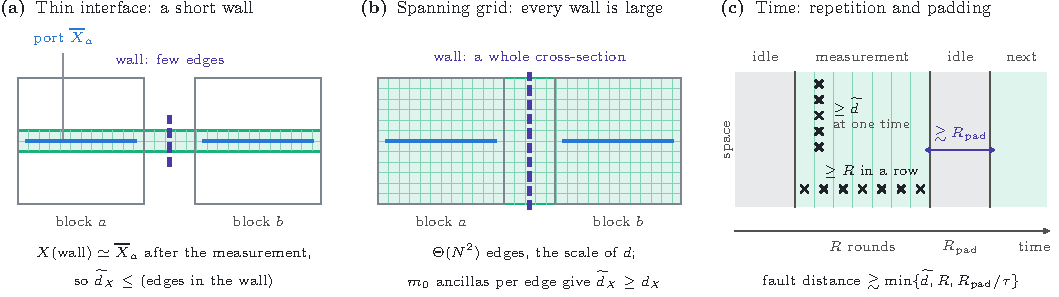
\includegraphics[width=\textwidth]{fault_distance_intuition.pdf}
\caption{Why the measurement keeps the fault distance, in a side view of two
blocks (squares) with their $X$ slab ports (blue) and the ancilla grid
(green).  (a) If the grid joins the blocks only through a thin bridge, $X$ on
a wall across the bridge (dashed) is equivalent to $\overline X_a$ once
$\overline X_a\overline X_b$ is measured, so a few faults cause a logical
error.  (b) If the grid fills both blocks, every wall between their ports is
a whole cross-section, with $\Theta(N^2)$ edges, the same scale as the code
distance; $m_0$ ancillas per edge make every wall at least as heavy as the
ports it separates, and the full distance is kept.  (c) In time, an
undetected error inside a measurement is either a logical at one time step,
with at least $\widetilde d$ faults, or one outcome wrong in each of the $R$
repeated rounds.  Idle rounds between operations force any pattern that links
two of them to stretch across the padding.}
\label{fig:fault-distance}
\end{figure*}

Four ingredients keep the distance.  First, the grid fills the
participating blocks, so every wall between their ports is a surface with
$\Omega(N^2)$ edges [Fig.~\ref{fig:fault-distance}(b)]; this is the constant
relative expansion of Eq.~\eqref{eq:grid-bound}, which the constant slab
thickness makes possible.  Second, carrying $m_0=\lceil2At\rceil$ parallel
ancillas on every grid edge multiplies every wall by $m_0$, so $\beta\ge1$
and Eq.~\eqref{eq:gauge-distance} gives $\widetilde d_X\ge d_X$: each
measurement keeps the full static distance at constant ancilla cost
(Supplemental Corollary~\ref{SM-cor:edge-multiplicity}).  Third, the
measurement is repeated in time [Fig.~\ref{fig:fault-distance}(c)].  A single
wrong outcome of one vertex star flips the reported product, so the new
checks are measured for $R=\Theta(d)$ rounds, and a wrong outcome that is
not repeated is caught by comparing consecutive rounds.  To flip the result
undetected, faults must corrupt the same outcome in every one of the $R$
rounds.  Williamson and Yoder proved the resulting fault-distance bound for
gauging \cite{WilliamsonYoderGauging}.  Because our operations start and end
in open idle rounds rather than at perfect boundaries, we give a short direct
proof (Supplemental Proposition~\ref{SM-prop:slice-bound}).  Split the faults
by type.  Faults of the measured type ($X$) leave, at the end, an error on
the data and a set of flipped edge readouts; together these form one
operator of the deformed code, which is a nontrivial logical whenever they
cause an error.  Every qubit of it carries at least one fault, so there are
at least $\widetilde d_X$ faults.  Faults of the other
type either leave a logical error on the data, again with at least $d_Z$
faults, or flip the reported outcome.  In that case either every one of the
$R$ rounds contains a wrong outcome, or a round without one shows that the
errors accumulated so far form a logical operator that anticommutes with the
measured one, with at least $d_Z$ faults.  Hence the measurement has fault
distance at least $\min\{\widetilde d_X,d_Z,R\}$, and exact minimization on
small instances shows that this bound is attained.  Fourth,
successive measurements on a block are separated by $\Theta(d)$ idle rounds,
so faults that straddle two operations also cost $\Omega(d)$
(Sec.~\ref{sec:ft-main}).

Resource transfer is the one place where blocks of different distance meet.
Joining a small block to a large one cannot expose the large block: the same
wall argument, applied to everything except the small block's own logical
qubits, shows that every other logical operator keeps the distance of the
larger block (Supplemental
Lemma~\ref{SM-lem:encoded-port-quotient}). The small courier blocks below
therefore carry only one traveling resource each, and their errors are
charged to distillation. Supplemental Table~\ref{SM-tab:distance-ledger}
lists the resulting bound for every operation: each logical qubit that is
read later, other than a resource in transit, is protected at every step by
fault distance $\Omega(d)$.


\subsection{Gates and encoded resources}
Pure-$X/Z$ measurements suffice for the logical gate set. A CNOT uses an
ancilla $a$ in $|+\rangle$ and the measurements
\begin{equation}
 Z_cZ_a\;(u),\qquad X_aX_t\;(v),\qquad Z_a\;(w),
 \label{eq:cnot}
\end{equation}
followed by the Pauli-frame update $Z_c^vX_t^{u\oplus w}$.
Outcome bit zero denotes eigenvalue $+1$.

For phase teleportation, prepare $a$ in $R_\theta|+\rangle$, where
$R_\theta=\operatorname{diag}(1,e^{i\theta})$, measure $Z_dZ_a$ with bit $m$
and $X_d$ with bit $n$, and retain $a$. The correction
\begin{equation}
 C_{mn}=R_{2\theta}^{m}Z_a^nX_a^m
 \label{eq:phase}
\end{equation}
produces $R_\theta|\psi\rangle$. For $\theta=\pi/2$ this consumes
$|Y\rangle=S|+\rangle$; for $\theta=\pi/4$ it consumes
$|A\rangle=T|+\rangle$, with a possible $S$ correction using one additional
$|Y\rangle$. Exchanging $X$ and $Z$ gives $S_X=HSH$, and
$SS_XS=e^{i\pi/4}H$. These identities generate Clifford+$T$ using the
one- and two-block measurements above. Complete branch maps and resource
counts appear in Supplemental Sec.~\ref{SM-sec:gates}.

A physical resource enters at a designated bare port. The raw qubit is
teleported into an encoded block by a joint $ZZ$ measurement and an $X$
readout. Its weight-one error class is the intentional resource degree of
freedom; all spectator logical classes retain distance $\Omega(d)$ in the
quotient by that class. Subsequent transfers use only encoded blocks, with
distances growing by fixed factors. We call this sequence an encoded courier.
Each courier block is dedicated to one traveling resource; its other logical
qubits are prepared in fixed states and never read.

The resource supply uses fixed Steane $7\!\to\!1$ and punctured Reed--Muller
$15\!\to\!1$ factories, implemented by the same logical primitives
\cite{BravyiKitaev,Reichardt,LitinskiMSD}.  Resource errors are modeled as
local-stochastic defective slots: a defective candidate may be in any state,
entangled with other candidates or with the environment.  Phase teleportation
with any such resource applies, relative to the ideal rotation, an operator in
$\operatorname{span}\{I,Z\}$ on the coordinate it feeds.  A predetermined
recovery therefore returns exactly the ideal output whenever at most one
coordinate of a run is defective, so each run always produces an output, and
the outputs are again a defective family with
\begin{equation}
 q_{r+1}\le C_{\rm dist}q_r^2.
 \label{eq:distill}
\end{equation}
The constant counts pairs among the fifteen principal and fifteen correction slots of a run, $C_{\rm dist}=\binom{30}{2}=435$.  Disjoint runs
use disjoint candidate sets; their errors need not be independent, and no
twirl or diagonal error basis is assumed. The raw
boundary, encoded transfers, and factories are included in the circuit
analysis rather than supplied as ideal external resources.

\section{Fault tolerance and resource scaling}
\label{sec:ft-main}
\subsection{From local distance to a complete circuit}
We consider local-stochastic Pauli circuit noise: any specified set $F_0$ of
fault mechanisms at distinct locations occurs with probability at most
$p^{|F_0|}$.  A round of check measurements has constant depth and uses only
nearest-neighbor gates on a finite ancilla schedule.  Each circuit fault acts
like at most $c_1=O(1)$ elementary faults of the simpler phenomenological
model, in which a fault is a data error or a wrong measurement outcome.  We
count faults in that model and divide by $c_1$ at the end.

The argument that the whole computation keeps fault distance $\Omega(d)$ has
a simple shape.  An undetected logical error needs a fault pattern that no
detector notices, that is, no comparison of consecutive outcomes and no
entry, exit, preparation, or readout check.  Split such a pattern into
connected pieces, where two faults are connected when they can trigger a
common detector; at least one piece causes the error.  A piece that lies
inside one operation and the idle rounds around it needs at least
$\min\{d,R\}$ faults, by Sec.~\ref{sec:distance-floor}.  Successive operations
on a block are separated by $R_{\rm pad}$ idle rounds.  Two connected faults
are at most $\tau=O(1)$ rounds apart, so a piece that reaches from one
operation to the next must stretch across the padding and needs about
$R_{\rm pad}/\tau$ faults.  Precisely, with $\delta_g^{\rm rel}$ the fault
distance of measurement window $g$ and $\delta_{\rm mem}^{\rm rel}$ that of
idle memory, both defined below, the composed phenomenological distance
satisfies
\begin{equation}
 f_{\rm ph}\ge\min\left\{
 \min_g\delta_g^{\rm rel},\delta_{\rm mem}^{\rm rel},
 1+\left\lfloor\frac{R_{\rm pad}-\tau}{\tau}\right\rfloor
 \right\},
 \label{eq:composition}
\end{equation}
with $\delta_g^{\rm rel}\ge\min\{\beta_0d,R_g\}$ for a window of $R_g$ rounds
and $\delta_{\rm mem}^{\rm rel}\ge d$.  Choosing $R_g$ and $R_{\rm pad}$ of
order $d$ makes every term $\Omega(d)$, and the bounded spread $c_1$ converts
this into a circuit-distance bound.

The technical work lies in making ``inside one operation'' precise without
assuming that each operation starts from a perfect state, since earlier
faults leave their traces.  We cut the schedule in time at idle rounds and
carry three pieces of data across each cut: the syndrome $s$ left by earlier
errors and the logical Pauli correction $\lambda$ accumulated so far, which
together describe the quantum state, and the outcomes $\rho$ of the last
measurement round, which the next detectors compare against.  The records
must be carried separately because a wrong outcome in the last round before
a cut changes $\rho$ but not the state.  With these three variables, adjacent
operations compose exactly; a direct simulation of an
idle$\,\to\,$gauging$\,\to\,$idle$\,\to\,$gauging$\,\to\,$idle schedule on
explicit layer-code blocks agrees with the composed map on every single
phenomenological fault mechanism, and gluing without $\rho$ fails.  Each
piece of a fault pattern is then judged by its effect \emph{relative} to the
same schedule without it: subtracting the fault-free evolution of the same
incoming data removes every dependence on earlier errors.  This includes a
less obvious one: when the logical representatives at two cuts differ by
stabilizers, the propagated frame acquires a term $Cs_{\rm in}$ linear in the
incoming syndrome.  A piece that lies between two cuts placed in idle
padding, with one round free of it before the right cut, leaves no syndrome
and no records at either cut, so its relative effect is its true effect and the window bounds
above apply to it (Supplemental Lemma~\ref{SM-lem:contained-cut}).

Resource errors need one more step, because the courier blocks have smaller
distance.  An error that a resource already carries is passed along with the
other incoming data.  A new error first created at encoded courier stage $j$
needs a connected fault pattern of size $\Omega(d_j)$ when that stage's
measurement and padding times are $\Theta(d_j)$; the raw injection stage is
charged separately, with a constant.  Distinct resources are kept far apart in
spacetime, so one short connected pattern cannot corrupt two of them.  The
reason is again the padding: a chain of connected faults can leave the
courier blocks of one resource only through its transfer into the factory
block, and from there it must stay on that block for the $R$ idle rounds
that separate the transfer from every other operation on it, whatever cells
it visits afterwards (Supplemental Lemma~\ref{SM-lem:resource-separation}).
A script builds a complete factory schedule by these rules, with cell reuse
and adaptive branches, and checks them and the resulting separation on it.
Summing
over the stages gives a raw-to-encoded resource error parameter
$q_0=O(\sqrt p)$ uniformly in the terminal distance, and
Eq.~\eqref{eq:distill} then suppresses the resource error quadratically.

Every detector has bounded support, so the graph that connects faults
through common detectors has bounded degree, uniformly over the finitely many
branches at adaptive steps.  The committed decoder chooses a minimum-cardinality fault set consistent with
the detector history through a fixed buffer beyond the commitment time.  A
wrong decision about a protected outcome requires a large connected set of
fault locations, a fixed fraction of which are actual faults.  Counting such
connected sets in a bounded-degree graph therefore yields a positive
threshold. This is an information-theoretic
decoder; efficient classical decoding is not assumed. Supplemental
Sec.~\ref{SM-sec:ft} gives the local detector, relative-distance, resource,
and cluster arguments in full.

\subsection{Architecture theorem}
The input family is a balanced good CSS LDPC family with boundedly dense
available sizes: every sufficiently large target length has an available
member within a fixed multiplicative factor. Fixed-degree Quantum Tanner
families provide the existential input used here
\cite{LeverrierZemorTanner,DinurLTC}. Let $A\subset\mathbb Z^3$ be the finite
allocated logical region, $W=|A|$, and $T$ the logical circuit depth. Allocated
working sites are included in $W$; physical gate ancillas and live factory
resources are included in the bound below.

To state the geometric overhead, partition the logical lattice into coarse
boxes of side $b(f)=\Theta(f^{1/6})$. Define $B_f(A)$ as the number of boxes
that meet $A$ but are not completely filled. This counts partial occupancy
at the block-packing scale, including boundaries, holes, and fragmentation.

\begin{theorem}[Universal fault-tolerant architecture]
\label{thm:architecture}
Use the explicit layer-code realization of Theorem~\ref{thm:slabs}, a
balanced good input family with boundedly dense sizes, and the local
measurement, resource, and extraction schedules described above. There are constants
$p_{\rm th},c,f_{\min}>0$ such that for $0<p<p_{\rm th}$ and target failure
$0<\varepsilon<1/2$, any finite nearest-neighbor three-dimensional logical
circuit can be simulated with
\begin{equation}
 f=\max\left\{f_{\min},
 \left\lceil\frac{c\log(WT/\varepsilon)}{\log(p_{\rm th}/p)}\right\rceil
 \right\},
 \label{eq:f}
\end{equation}
using
\begin{align}
 Q_{\rm phys}&=O\!\left(Wf+(B_f(A)+1)f^{3/2}\right),
 \label{eq:space}\\
 D_{\rm phys}&=O(Tf^{3/2}\Psi),\qquad \Psi=O(f^{\log_215}).
 \label{eq:depth}
\end{align}
Persistent data remain in layer-code blocks, and physical operations use
nearest-neighbor connectivity. For a connected bounded-aspect logical box,
\begin{equation}
 Q_{\rm phys}=O(Wf+f^{3/2}).
 \label{eq:box-space}
\end{equation}
\end{theorem}

The scaling follows directly from the code parameters. Choose
$d=\Theta(f)$ and measurement, padding, and commitment buffers of order $f$.
Equation~\eqref{eq:parameters} then gives
\begin{equation}
 N=\Theta(\sqrt f),\qquad K=\Theta(\sqrt f),\qquad n=\Theta(f^{3/2}).
 \label{eq:chosen-size}
\end{equation}
A full coarse logical box fits into one cell. Counting full and partial
boxes requires $O(W/K+B_f(A)+1)$ data/factory cells. Multiplication by
$n$ proves Eq.~\eqref{eq:space}. Neighboring logical sites map to the same
cell or adjacent cells, and a bounded coloring schedules inter-cell gates.

\begin{figure*}[t]
\centering
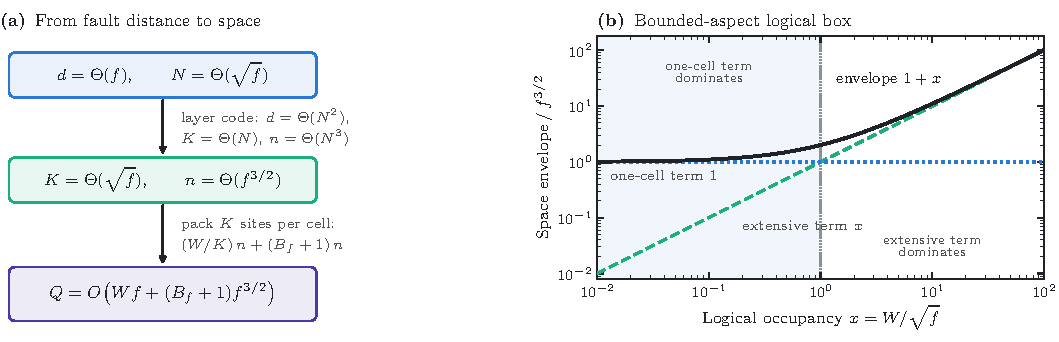
\includegraphics[width=\textwidth]{revision_resources.pdf}
\caption{Origin and crossover of the resource bound. (a) Target fault distance
$f$ fixes the cell parameters; packing $K=\Theta(\sqrt f)$ logical sites per
cell yields an extensive $Wf$ term plus the cost of partially occupied cells.
(b) For bounded-aspect boxes, the normalized scaling envelope is proportional
to $1+x$, where $x=W/\sqrt f$. The one-cell term dominates for $x\ll1$ and
the extensive term for $x\gg1$. Constants are suppressed: this is an
illustration of the asymptotic bound, not a numerical qubit estimate.}
\label{fig:resources}
\end{figure*}

For a bounded-aspect logical box,
$B_f(A)=O((W/\sqrt f)^{2/3}+1)$, so the partial-cell term is absorbed into
Eq.~\eqref{eq:box-space}. Figure~\ref{fig:resources} shows the crossover at
$W\sim\sqrt f$. Thin or fragmented regions retain the general correction.

For time, a distilled resource takes $O(f\Psi)$ rounds, where $\ell$
distillation levels give $\Psi=O(15^\ell)$ and $2^\ell=O(f)$. One logical
layer requires $O(K)$ resources per data block, and serial production gives
$O(Kf\Psi)=O(f^{3/2}\Psi)$ rounds per layer, that is
$O(f^{3/2+\log_215})\subseteq O(f^{5.41})$. This serial schedule is chosen
to keep the space bound; parallel factories would trade space for depth. A depth-first factory schedule
stores $O(\ell)$ candidates at once, which fits within the reserved logical
capacity. The complete location count is polynomial in $f$ times
$WT\Psi$; the exponential cluster bound and final-resource union bound are
both at most $\varepsilon/2$ for the choice in Eq.~\eqref{eq:f}.
The detailed theorem and constant ledger appear in Supplemental
Theorem~\ref{SM-thm:A24}.

The depth deserves as much attention as the space.  Per logical layer the
minimal-space schedule takes $O(Kf\Psi)=O(f^{3/2+\log_215})$ rounds, against
$O(f)$ for lattice surgery.  With $P$ factories per cell the space becomes
$O(WfP+f^{3/2})$ and the depth $O(TKf\Psi/P)$, so qubit-time is unchanged: the
serial schedule minimizes space, not space--time volume.  A concrete estimate
with stated constants, explicit integer allocations, and distances chosen
from each schedule's complete runtime (Supplemental
Sec.~\ref{SM-sec:resource-estimate}) makes the scales explicit.  For $W=100$
sites, $T=10^6$ layers, $\varepsilon=10^{-2}$, $p=10^{-3}$, and injected
resource error $10^{-2}$, the always-output distillation covered by the
theorem does not converge: Eq.~\eqref{eq:distill} requires an injected error
below $1/C_{\rm dist}\approx2.3\times10^{-3}$, and even the ideal factory,
whose error map starts at $105q_c^2$ with the per-coordinate error $q_c$
including the $S$ corrections, requires about $5\times10^{-3}$.  With
optimistic postselected distillation, which the theorem does not cover, the
serial layer-code schedule needs about $10^9$ qubits for two months, against
$4\times10^5$ qubits for three days for a serial surface-code layout and
$2\times10^8$ qubits for $23$\,s for a throughput-limited one.  At these
distances a layer-code block holds one to three logical qubits; with the same
accounting on both sides it stores a logical more cheaply than a surface-code
patch only for $d\gtrsim1100$ (between about $600$ and $2300$ across the
distance scenarios).
The asymptotic advantage is therefore far from the practical regime until
these constants, and the distillation protocol, improve.

The same architecture argument applies to any three-dimensional CSS
family with the parameter scaling in Eq.~\eqref{eq:parameters}, bounded
local density and aspect ratio, boundedly dense sizes, and uniformly
slab-supported pure logicals; the explicit realization supplies all of these. These are substantive geometric assumptions;
Supplemental Corollary~\ref{SM-cor:slab-transfer} states the transfer precisely.

\section{Port packing and shallow logical gates}
\label{sec:structure}
Slab mobility also constrains how logical information can be spatially
accessible. For a region $A$, let $g_X(A)$ be the dimension of the pure-$X$
logical space supported in $A$, and define $g_Z(B)$ analogously. The rank
$r(A,B)$ of their commutation pairing obeys
\begin{equation}
 \max\{0,g_X(A)+g_Z(B)-K\}\le r(A,B)\le |A\cap B|.
 \label{eq:overlap}
\end{equation}
The upper bound follows because all cross commutation factors through the
intersection; the lower bound follows from nondegeneracy of the full
logical $X/Z$ pairing.

If $A_1,\ldots,A_{r_X}$ are disjoint complete $X$ ports and
$B_1,\ldots,B_{r_Z}$ disjoint complete $Z$ ports, summing
Eq.~\eqref{eq:overlap} over all pairs gives the crossbar bound
\begin{equation}
 r_Xr_ZK\le n.
 \label{eq:crossbar}
\end{equation}
Every crossing carries rank $K$, and the crossings are pairwise disjoint.
For the balanced layer-code slabs,
$r_X,r_Z=\Theta(N)$, $K=\Theta(N)$, and $n=\Theta(N^3)$, so the bound is
saturated up to constants. Each transverse intersection has size
$\Theta(K)$, while each complete slab has size $\Theta(d)$. Thus the cubic
physical size is optimal among CSS families required to provide
$\Theta(K)$ disjoint complete ports in both polarizations. This is a bound
on simultaneous spatial access, distinct from a storage lower bound.

There is a complementary constraint on unitary processing. Pair the $i$th
$X$-slab representative and the $i$th $Z$-slab representative of any logical
Pauli. Each qubit belongs to at most two resulting representatives, giving
disjointness $\Delta=\Omega(N)$. The logical-weight bounds sharpen this to
\begin{equation}
 \Delta=\Theta(N),\qquad
 d_\downarrow=\Theta(N^2),\qquad d_\uparrow=\Theta(N^2),
 \label{eq:disjoint}
\end{equation}
where $d_\downarrow$ and $d_\uparrow$ are the smallest and largest minimum
weights among nontrivial logical Pauli classes. The
Jochym-O'Connor--Kubica--Yoder criterion then forces every fixed-depth,
bounded-arity, code-preserving unitary on a sufficiently large static block
to be logical Clifford \cite{JochymDisjointness}. The result holds even
without geometric locality of those gates. The architecture uses adaptive
measurements, resource states, and changing codes, which lie outside that
unitary setting. Complete packing and disjointness proofs are in Supplemental
Secs.~\ref{SM-sec:symplectic-overlap} and~\ref{SM-sec:disjointness-obstruction}.

\section{Finite numerical evidence}
\label{sec:numerics-main}
The supplied simulations test finite interfaces in the construction.  Three
campaigns run complete circuits on explicit layer-code blocks
(Fig.~\ref{fig:two-block}); the largest campaign, which shows a clean
crossing, uses surface codes.
That campaign follows a single encoded planar surface code of distance
$L$, with $n=L^2+(L-1)^2$ data qubits, through an algebraic base-code
$\rightarrow$ gauged-strip $\rightarrow$ base-code circuit, without
resetting the data between stages. The gauged strip is a path of $L$
ancilla qubits attached to a weight-$L$ logical representative, so the
campaign tests the gauging interface and the detector bookkeeping of a code
switch rather than the layer-code geometry. Its entry and exit satisfy the binary
stabilizer transition identities. Noisy repeated extraction produces one
detector history, decoded by minimum-weight perfect matching from exact
graphlike detector error models.

The SI1000-like model uses two-qubit depolarizing strength $p$, single-qubit
and ordinary idle strength $p/10$, measurement flips $5p$, reset noise $2p$,
and data idle-wait noise $2p$. The archived campaign comprises 255 parameter
points and $4.534\times10^6$ shots for sizes $L=3,5,7,9,11$ and gauged
durations $G=d,2d,3d$, where $d=L$ is the code distance. All 15 noiseless controls have zero failures.

For every duration, the failure rate decreases monotonically with $L$ across
all five sizes at every tested $p\le0.004$ (Supplemental
Fig.~\ref{SM-fig:supp-continuous}). Consecutive-size Wilson intervals are separated
at every tested $p$ from $0.0025$ to $0.00375$ for all three durations. At $p=0.0035$, increasing $L$ from 3 to 11 reduces the
failure rate from $0.1111$ to $0.0324$ for $G=d$, and from $0.1326$ to
$0.0428$ for $G=3d$. At $p=0.0015$ and $G=d$, the reduction is approximately
$6.5\times10^2$.

The smallest-versus-largest crossing medians are
$4.471$, $4.431$, and $4.328\times10^{-3}$ for $G=d,2d,3d$, with conditional
95\% posterior bands $[4.426,4.522]$, $[4.392,4.466]$, and
$[4.265,4.393]\times10^{-3}$. Tripling the gauged duration shifts the median
by about 3.2\%. These are finite-size diagnostics of a surface-code gauging model; they do
not estimate the architecture theorem's asymptotic threshold, which concerns
layer codes and a committed minimum-weight decoder.

\begin{figure*}[t]
\centering
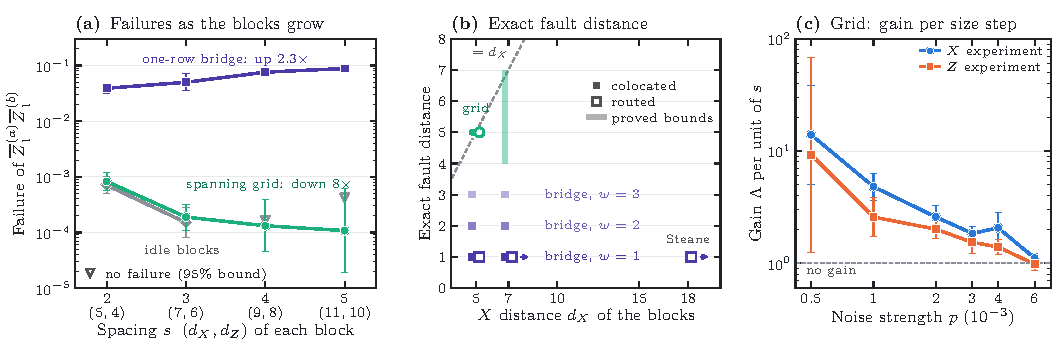
\includegraphics[width=\textwidth]{two_block_main.pdf}
\caption{Two-block logical measurement on explicit layer-code blocks: the
cut obstruction at scale, in simulation (the hardware counterpart is
Fig.~\ref{fig:hardware}).  (a)~Failure of the measured pair
$\overline Z_1^{(a)}\overline Z_1^{(b)}$ at $p=10^{-3}$ as the block spacing
$s$ grows, through a one-row bridge (violet) and a spanning grid (aqua), and
for the same blocks left idle (grey), with Wilson 95\% intervals (open
triangles: Wilson upper ends of zero counts).  (b)~Exact circuit fault
distance of the measured pair against the $X$ distance of the blocks,
computed by CP-SAT.  Filled: colocated ancillas at $s=2,3$; open: routed
nearest-neighbor extraction at $s=2$ with the $[[4,2,2]]$, band and Steane
inputs, whose blocks have $X$ distance $5$, at least $7$ and at least $18$
(arrows); bar: the proved lower bound and the weight of an undetectable
pattern where the solver stopped.  Through a bridge of $w$ rows the distance
stays at $w$ while $d_X$ grows; through the grid it equals $d_X$ (dashed)
where it is resolved.  (c)~Factor $\Lambda$ by which each unit of spacing
suppresses failures of any observable through the spanning grid, from a
weighted fit over $s=2$ to $5$, with 95\% intervals.}
\label{fig:two-block}
\end{figure*}

A complete joint measurement on explicit layer-code blocks tests what the
surface-code campaigns cannot: the reported bit, both logical sectors,
spectator logicals, and an entangled input.  Two $[[4,2,2]]$-input blocks
($n=224$, two logical qubits each, distances $5$ and $4$) measure
$\overline X_1^{(a)}\overline X_1^{(b)}$ by gauging on a planar grid attached
to their single-layer slabs, with ancilla-based extraction of every check and
uniform circuit noise.  Each logical qubit starts maximally entangled with a
noiseless reference, and eight observables certify the output Choi state.
Without noise every detector and observable is deterministic, so the circuit
implements the projective measurement with the correct outcome and leaves the
spectators untouched.  We then compute, exactly, the minimum number of faults
that flips each observable undetectably.  With a bridge of $w=1,2,3$ grid rows
between the blocks, the fault distance of
$\overline Z_1^{(a)}\overline Z_1^{(b)}$ is exactly $w$; for $w=1$ a single fault
suffices [Fig.~\ref{fig:two-block}(b)].  This is the cut obstruction of
Sec.~\ref{sec:distance-floor} at circuit level.  A grid spanning both blocks restores it to exactly $5$, the
blocks' $X$ distance, while the fault distances of the reported bit, set by
the number of rounds, and of the spectators do not depend on the interface
(Supplemental Sec.~\ref{SM-sec:two-block}).

A second campaign repeats the measurement on blocks of spacing $s=2$ to $5$
(block distances up to $d_X=11$, up to $1400$ qubits per block), with $2s+1$
rounds per phase and $3.0\times10^6$ shots, decoded in each CSS sector
separately (Supplemental Sec.~\ref{SM-sec:two-block-scaling}); on identical
shots the full-model BP+LSD decoder of the first experiment (Supplemental
Table~\ref{SM-tab:two-block}) fails less often through the grid
(half as often in the $X$ experiment) and about as often through the bridge,
so the contrast below is, if anything, understated.  At $p=10^{-3}$ the failure rate of
$\overline Z_1^{(a)}\overline Z_1^{(b)}$ through the one-row bridge rises from
$3.9\%$ at $s=2$ to $8.8\%$ at $s=5$, because the undetectable bridge fault
has more rounds in which to occur, while through the spanning grid it falls
from $8.2\times10^{-4}$ to about $10^{-4}$ and agrees with the same blocks
left idle [Fig.~\ref{fig:two-block}(a)].  For the spanning grid each unit of
spacing suppresses failures by a factor $4.8$ in the $X$ experiment and $2.6$
in the $Z$ experiment at $p=10^{-3}$, falling to one near
$p\approx6\times10^{-3}$ [Fig.~\ref{fig:two-block}(c) and Supplemental
Fig.~\ref{SM-fig:two-block-scaling}].  At $s=3$ the fault distance of
$\overline Z_1^{(a)}\overline Z_1^{(b)}$ through a bridge of $w=1,2,3$ rows is
still exactly $w$, although the blocks' $X$ distance is now $7$.

A third campaign replaces the colocated ancillas by the routed
nearest-neighbor schedule of Supplemental
Proposition~\ref{SM-prop:nn-extraction}, with SWAP-shuttled ancillas,
colored conflict classes, and idle noise in every time step, and grows the
input at $s=2$: $[[4,2,2]]$, a six-qubit band code, and the Steane code,
giving blocks of $224$, $720$ and $1792$ qubits and circuits of up to
$16{,}293$ qubits (Supplemental Sec.~\ref{SM-sec:two-block-routed}).  Without
noise all $28$ measurement circuits implement the measurement exactly, and
the $12$ idle controls also give silent detectors and correct observables.  Through the one-row bridge the
fault distance of $\overline Z_1^{(a)}\overline Z_1^{(b)}$ is exactly $1$ for
all three inputs, although the blocks' $X$ distance grows from $5$ to at
least $18$ [Fig.~\ref{fig:two-block}(b)].  On the $[[4,2,2]]$ blocks with $R=5$ rounds per phase
the spanning grid gives exactly $5$, the same as the blocks left idle;
through both interfaces the reported bit has exactly $5=R$, and the
spectator $X$ frames have exactly $4=d_Z$, as in idle memory.  Where both are
resolved, routing leaves the distances of the colocated circuit unchanged.
On the band blocks the reported bit has an undetectable pattern of weight $6$
at $R=7$.  The block itself explains this weight: the lightest $Z$-type
operator that anticommutes with the measured logical has weight $6$, so no
schedule gives the bit more than $\min\{R,6\}$; whether routing adds lighter
patterns is open.  At the tested noise strengths the sampled
failure rates of these long routed circuits do not distinguish the
interfaces, so we use only their exact fault distances.

Complementary memory, local-gauging, factory, and stage-composed
tests are reported in Supplemental Sec.~\ref{SM-sec:supp-numerics}. The
deterministic checks cover the complete-code slab certificate, refinement
identities, gate maps, 10,008 single-location faults in the finite extraction
catalog, and the thin-versus-thick interface comparison of
Sec.~\ref{sec:distance-floor}. These checks support the individual
interfaces and remain separate from the arbitrary-size proofs.

\section{Hardware demonstrations}
\label{sec:hardware-main}
Three mechanisms of Sec.~\ref{sec:distance-floor} are small enough to run on
present superconducting processors: the cut obstruction, its removal by
parallel ancillas, and the protection of the reported bit by repeated
rounds.  We ran them on the 54-qubit IQM Emerald processor through the Open
Quantum platform~\cite{OpenQuantum2026} and on the 156-qubit IBM Heron
processors \texttt{ibm\_fez} and \texttt{ibm\_kingston}, with
\hwTotalShots~million analyzed samples.  The top row of
Fig.~\ref{fig:hardware} shows what was run and the bottom row what was
measured.  The blocks are three-qubit repetition codes, not layer codes, so
these runs test the mechanisms and not the architecture.  Apart from the
routed \texttt{ibm\_fez} circuits, every circuit was placed without SWAP
gates [Fig.~\ref{fig:hardware}(a) and Supplemental
Fig.~\ref{SM-fig:hardware-chips}], and before each submission the exact
circuit fault distance of the circuit as sent was computed.  A script
computes every number below from the archived raw outputs (Supplemental
Sec.~\ref{SM-sec:hardware}).

\begin{figure*}[t]
\centering
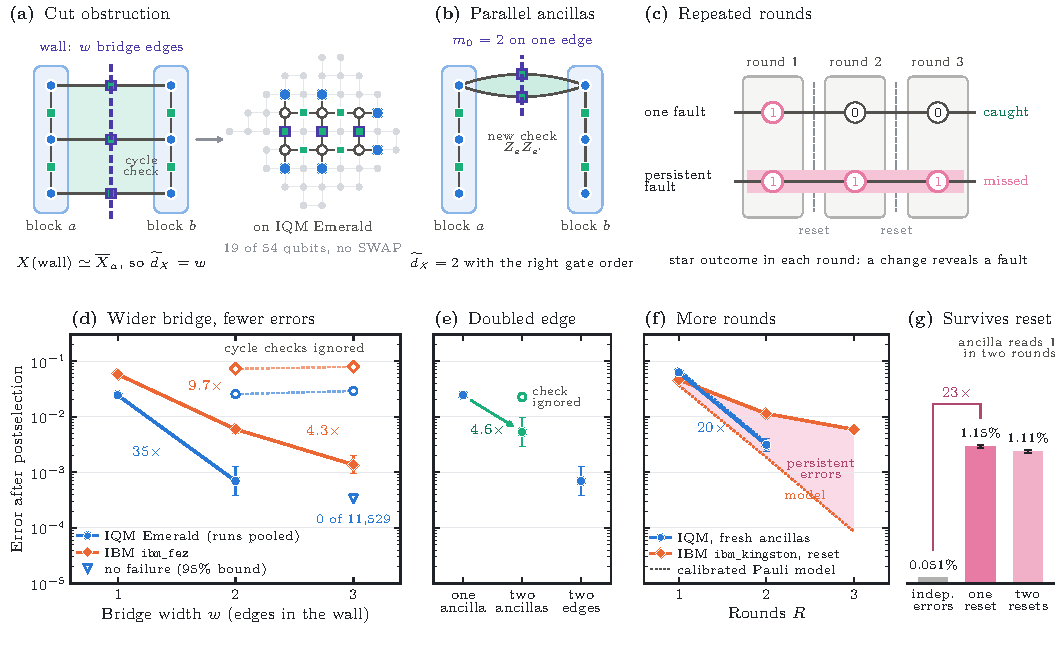
\includegraphics[width=\textwidth]{hardware_overview.pdf}
\caption{Hardware demonstrations of the three distance mechanisms.  Top row:
what was run (schematics).  (a)~Two three-qubit blocks (blue) joined by a
bridge of $w$ edges, each with an edge ancilla (aqua squares); $X$ on the
wall of bridge edges (violet) is equivalent to $\overline X_a$, so the
deformed $X$ distance and the exact circuit fault distance are both $w$.
Shaded: the cycle checks that the extra bridge edges create.  Right: the
circuit for $w=3$ as placed on IQM Emerald, with the couplers it uses.
(b)~Two parallel ancillas on one bridge edge ($m_0=2$) add the two-edge check
$Z_eZ_{e'}$.  (c)~A wrong star outcome in one round is revealed by the change
in the next round; a fault that persists across rounds repeats the same
wrong outcome and is missed.  Bottom row: what was measured, as the error
after postselection on every detector, with Wilson 95\% intervals (open
triangle: Wilson upper end of a zero count).  (d)~IQM runs pooled; open
symbols: the same samples with the cycle checks ignored.  (e)~IQM, one bridge
edge with one or two ancillas, and two bridge edges; open symbol: the
two-edge check ignored.  (f)~Reported-bit error against the number of rounds
$R$, with the calibrated Pauli models (dotted); IQM uses fresh ancillas in
every round, \texttt{ibm\_kingston} measures and resets them.  Shaded: the
excess over the model (run A).  (g)~Rate at which a check ancilla on
\texttt{ibm\_kingston} (run B) reads 1 in two consecutive rounds with no data error to
explain it, against the rate that independent errors give, with one or two
resets between rounds.  Every run separately: Supplemental
Fig.~\ref{SM-fig:hardware-sm}.}
\label{fig:hardware}
\end{figure*}

\paragraph{Cut obstruction.}
Two blocks with $Z$ checks $Z_0Z_1$, $Z_1Z_2$ and
$\overline X=X_0X_1X_2$ start in $|000\rangle$ and $\overline X_a\overline
X_b$ is measured by gauging on a graph whose bridge between the blocks has
$w$ edges, so that $X$ on the bridge is a logical of weight $w$
[Eq.~\eqref{eq:cut-obstruction}]; the deformed $\overline Z_a\overline Z_b$
must stay $+1$.  The postselected error falls \hwIQMfold-fold, from
\hwIQMwOne\% at $w=1$ to \hwIQMwTwo\% at $w=2$, on IQM (pooled over three runs
on two sets of qubits; $p\le\hwIQMpOneTwo$ in each of the two runs with both
widths), and from \hwIBMwOne\% to \hwIBMwTwo\% and \hwIBMwThree\% at
$w=1,2,3$ on IBM, by factors of \hwIBMfoldOneTwo{} and \hwIBMfoldTwoThree{}
[Fig.~\ref{fig:hardware}(a,d)].  When the cycle checks that the extra bridge
edges create are ignored, the error returns to the width-one level
(\hwIQMctrl\% on IQM, \hwIBMctrl\% on IBM), so the gain comes from the larger
wall and not from discarding more samples.  On IQM, width three had no
failure in \hwIQMwThreeKept{} kept samples, but its difference from width two
is not significant ($p=\hwIQMpTwoThree$, in a test fixed before the run).

\paragraph{Parallel ancillas.}
Two parallel ancillas on a single bridge edge ($m_0=2$) give \hwMult\%
instead of \hwIQMwOne\%, a \hwMultFold-fold gain ($p=\hwMultP$), and
\hwMultCtrl\% when the new two-edge check is ignored
[Fig.~\ref{fig:hardware}(b,e)].  The first CNOT order we tried had circuit
fault distance one: a fault on the vertex ancilla between its two bridge
CNOTs put $X$ on both parallel edges, which the two-edge check cannot see.
Separating the two CNOTs restores distance two.  This is the constant-factor
loss from circuit faults that Sec.~\ref{sec:ft-main} allows for; a suitable
CNOT order avoids it.

\paragraph{Repeated rounds and errors that survive a reset.}
For the reported bit we use phase-flip blocks ($d_Z=3$) joined by one edge
and measure the two vertex stars and the four block checks in $R$ rounds
[Fig.~\ref{fig:hardware}(c)].  With fresh ancillas in each round (IQM, which
does not allow a measured qubit to be reused), the error falls
\hwRndIQMfold-fold, from \hwRndIQMOne\% at $R=1$ to \hwRndIQMTwo\% at $R=2$,
close to the model's \hwRndIQMModelOne\% and \hwRndIQMModelTwo\%
($p=\hwRndIQMp$, fixed in advance).  On IBM, where the ancillas are measured
and reset between rounds, it falls from \hwRndIBMOne\% to \hwRndIBMTwo\% and
\hwRndIBMThree\% for $R=1,2,3$ (both steps $p\hwRndIBMpOneTwo$, fixed in
advance), but far less than the calibrated model predicts (\hwRndIBMModelTwo\%
and \hwRndIBMModelThree\% at $R=2,3$); at $R=3$ the error is
\hwRndIBMModelRatio~times the prediction [Fig.~\ref{fig:hardware}(f)].  The
cause is an ancilla error that survives the reset: a check ancilla reads 1 in
two consecutive rounds, with no data error to explain it, in \hwPersSingle\%
of samples, \hwPersRatio~times the rate that independent errors give, and a
second reset removes only \hwPersRel\% of these events ($p=\hwPersP$)
[Fig.~\ref{fig:hardware}(g)].  Such a fault, most likely leakage, corrupts the
same outcome in every round.  It lies outside the local-stochastic model of
Sec.~\ref{sec:ft-main}, which charges every round separately.

\paragraph{What the runs show.}
Together, the runs reproduce at small scale the three facts that the distance
argument of Sec.~\ref{sec:distance-floor} combines: the smallest wall bounds
the distance of a joint measurement (as Fig.~\ref{fig:two-block} shows in
simulation on layer-code blocks), parallel ancillas widen every wall that
crosses their edge, and repeated rounds protect the reported bit.  They also
show which assumption of the theorem present hardware does not meet: faults
that persist across rounds.  They do not test layer codes, the grid
expansion, the threshold, or the resource scaling, which need far larger
devices.

\section{Discussion}
The main architectural contribution is a local route from layer-code storage
to universal processing. Prefix-parity repair exposes logical operators in
single-layer slabs of an explicit realization; grid gauging turns those slabs into protected
measurements; and a composed detector schedule supports resource transfer
and distillation in the same geometry. Because a layer-code distance is
comparable to the area of a block face, every joint measurement must cross a
constant fraction of that face; a thick grid does so and, with a constant
ancilla multiplicity, keeps the full distance, whereas a thin measurement
layer cannot.  Simulations on layer-code blocks and small hardware runs show
this contrast (Figs.~\ref{fig:two-block} and~\ref{fig:hardware}).  For
bounded-aspect logical regions,
the resulting space bound separates an extensive $Wf$ cost from the minimum
$f^{3/2}$ cost of one encoded cell.

The port-packing result gives a second interpretation of the layer-code
parameters. Their cubic physical volume supports linearly many disjoint
complete ports of each polarization, saturating the crossbar bound. Growing
mobility also explains why adaptive measurement and resource injection are
natural tools: shallow unitaries preserving a static large block are restricted
to the Clifford group.

The next steps are a practical decoder for deformation histories, with
changing checks, inherited frames and records, and joint measurements (the
layer-code decoders of Ref.~\cite{GuRandomLayerCodes2026} are a natural starting
point, although their memory guarantees do not yet cover code switching);
routed circuit-level benchmarks on inputs that grow into the balanced regime,
with a shorter routed schedule and a decoder close to minimum weight; bounds
on how many logical measurements can share
the slab interfaces, compared with parallel code surgery
\cite{CowtanParallelSurgery} under three-dimensional locality; and factories
whose constants make the space--time estimate competitive, possibly in a
different code with a protected local transfer. Random
layer codes built from random CSS inputs \cite{GuRandomLayerCodes2026} are a
natural candidate for reducing those constants; the explicit realization
applies to any CSS input, but the resource accounting would need their
parameter scaling. The present theorem uses minimum-weight committed decoding and
local-stochastic Pauli noise. Extensions to coherent or leakage noise require
an additional fault-path analysis; the IBM runs of
Sec.~\ref{sec:hardware-main} show that ancilla errors that persist across
rounds already limit the benefit of repeated rounds on present hardware, so
leakage reduction would belong in any implementation of the extraction
schedule.  Deterministic selection of the input
component codes is a separate constructive problem. The storage benchmark in
Supplemental Sec.~\ref{SM-app:storage-details} makes the restricted regime for
comparison with an extensive lower bound explicit, including the condition
$W=\Omega(\sqrt f)$ when the one-cell term is to be subleading.

\section*{Data availability}
The simulation datasets, finite algebraic certificates, verification scripts,
and figure-generation code are included in the accompanying source and
reproducibility package. The Supplemental Material describes the noise models,
decoders, stopping rules, and scope of each dataset.  The hardware circuits,
job identifiers, raw outcomes, calibration snapshots, and analysis scripts are
in the folder \texttt{hardware} of the package.

\begin{acknowledgments}
The author thanks Dominic J. Williamson for helpful correspondence. Williamson
pointed out that adding logical-measurement layers to a layer code can, in
principle, reduce its fault distance, noted that this question had been left
open in an earlier idea of performing universal computation on layer codes by
adding such layers, and suggested that random layer codes
\cite{GuRandomLayerCodes2026} may be useful here.
Section~\ref{sec:distance-floor} and the corresponding supplemental results
(the cut obstruction, the edge-multiplicity corollary, the encoded-port
quotient lemma, and the distance ledger) were added in response.  He later
suggested that the junction construction and the fault-distance argument be
explained in plainer terms, and Secs.~\ref{sec:slabs}, \ref{sec:measurements},
and~\ref{sec:ft-main}~A were rewritten for that purpose.  The
correspondence did not include a detailed review of the proofs, and any
errors are the author's own.  The IQM experiments used the Open Quantum
platform~\cite{OpenQuantum2026}.  We acknowledge the use of IBM Quantum
services for this work.  The views expressed are those of the author, and do
not reflect the official policy or position of IBM or the IBM Quantum team.
\end{acknowledgments}

\section*{Acknowledgment of AI assistance}
Claude Code assisted with manuscript organization, language editing, figure
preparation, and scripts from the supplied research materials and numerical
data.

\begin{thebibliography}{99}
\bibitem{WilliamsonBaspinLayerCodes}
D. J. Williamson and N. Baspin, Layer codes, Nat. Commun. \textbf{15}, 9528 (2024), \href{https://arxiv.org/abs/2309.16503}{arXiv:2309.16503}.

\bibitem{WilliamsonYoderGauging}
D. J. Williamson and T. J. Yoder, Low-overhead fault-tolerant quantum computation by gauging logical operators, Nat. Phys. \textbf{22}, 598 (2026), \href{https://arxiv.org/abs/2410.02213}{arXiv:2410.02213}.

\bibitem{CowtanParallelSurgery}
A. Cowtan, Z. He, D. J. Williamson, and T. J. Yoder, Parallel logical measurements via quantum code surgery, PRX Quantum \textbf{7}, 020325 (2026), \href{https://doi.org/10.1103/gj8x-n5gg}{doi:10.1103/gj8x-n5gg}.

\bibitem{YuanParsimonious2026}
A. C. Yuan, A. Cowtan, Z. He, T.-C. Lin, and D. J. Williamson, Parsimonious quantum low-density parity-check code surgery, \href{https://arxiv.org/abs/2603.05082}{arXiv:2603.05082} (2026).

\bibitem{IdeHomological}
B. Ide, M. G. Gowda, P. J. Nadkarni, and G. Dauphinais, Fault-tolerant logical measurements via homological measurement, Phys. Rev. X \textbf{15}, 021088 (2025), \href{https://doi.org/10.1103/PhysRevX.15.021088}{doi:10.1103/PhysRevX.15.021088}.

\bibitem{BerentLiftedSurgery}
L. Berent, L. Z. Cohen, and A. O. Quintavalle, Lifted surgery: Fast processing with QLDPC codes, \href{https://arxiv.org/abs/2609.11723}{arXiv:2609.11723} (2026).

\bibitem{SwaroopAdapters}
E. Swaroop, T. Jochym-O'Connor, and T. J. Yoder, Universal adapters between quantum low-density parity-check codes, PRX Quantum \textbf{7}, 010324 (2026), \href{https://arxiv.org/abs/2410.03628}{arXiv:2410.03628}.

\bibitem{HeExtractors}
Z. He, A. Cowtan, D. J. Williamson, and T. J. Yoder, Extractors: qLDPC architectures for efficient Pauli-based computation, \href{https://arxiv.org/abs/2503.10390}{arXiv:2503.10390} (2025).

\bibitem{ZhangGoodQLDPC}
G. Zhang, Y. Zhu, and Y. Li, Accelerating fault-tolerant quantum computation with good quantum low-density parity-check codes, PRX Quantum \textbf{7}, 033012 (2026), \href{https://doi.org/10.1103/3fj5-gn1h}{doi:10.1103/3fj5-gn1h}.

\bibitem{MalcolmEfficientQLDPC}
A. J. Malcolm, A. N. Glaudell, P. Fuentes, \emph{et al.}, Computing efficiently in QLDPC codes, Nat. Commun. \textbf{17}, 7286 (2026), \href{https://doi.org/10.1038/s41467-026-73061-9}{doi:10.1038/s41467-026-73061-9}.

\bibitem{BPT}
S. Bravyi, D. Poulin, and B. Terhal, Tradeoffs for reliable quantum information storage in 2D systems, Phys. Rev. Lett. \textbf{104}, 050503 (2010), \href{https://arxiv.org/abs/0909.5200}{arXiv:0909.5200}.

\bibitem{HorsmanLatticeSurgery}
D. Horsman, A. G. Fowler, S. Devitt, and R. Van Meter, Surface code quantum computing by lattice surgery, New J. Phys. \textbf{14}, 123011 (2012), \href{https://arxiv.org/abs/1111.4022}{arXiv:1111.4022}.

\bibitem{LitinskiSurgery}
D. Litinski, A game of surface codes: large-scale quantum computing with lattice surgery, Quantum \textbf{3}, 128 (2019), \href{https://arxiv.org/abs/1808.02892}{arXiv:1808.02892}.

\bibitem{VasmerBrowne}
M. Vasmer and D. E. Browne, Three-dimensional surface codes: Transversal gates and fault-tolerant architectures, Phys. Rev. A \textbf{100}, 012312 (2019), \href{https://arxiv.org/abs/1801.04255}{arXiv:1801.04255}.

\bibitem{PattisonHierarchical}
C. A. Pattison, A. Krishna, and J. Preskill, Hierarchical memories: Simulating quantum LDPC codes with local gates, Quantum \textbf{9}, 1728 (2025), \href{https://arxiv.org/abs/2303.04798}{arXiv:2303.04798}.

\bibitem{ChoeKoenigLocal}
S. H. Choe and R. K\"onig, How to fault-tolerantly realize any quantum circuit with local operations, \href{https://arxiv.org/abs/2402.13863}{arXiv:2402.13863} (2024).

\bibitem{BaspinWire}
N. Baspin and D. J. Williamson, Wire codes, Quantum \textbf{10}, 2083 (2026), \href{https://arxiv.org/abs/2410.10194}{arXiv:2410.10194}.

\bibitem{YangPlanar}
Y. Yang, G. Zhang, and Y. Li, Planar fault-tolerant logical measurements with low qubit overhead, npj Quantum Inf. (2026), \href{https://doi.org/10.1038/s41534-026-01310-2}{doi:10.1038/s41534-026-01310-2}, \href{https://arxiv.org/abs/2506.18061}{arXiv:2506.18061}.

\bibitem{GottesmanFTThreshold}
D. Gottesman, Fault-tolerant quantum computation with constant overhead, Quantum Inf.\ Comput.\ \textbf{14}, 1338 (2014), \href{https://arxiv.org/abs/1310.2984}{arXiv:1310.2984}.

\bibitem{KovalevPryadko}
A.~A. Kovalev and L.~P. Pryadko, Fault tolerance of quantum low-density parity check codes with sublinear distance scaling, Phys.\ Rev.\ A \textbf{87}, 020304(R) (2013).

\bibitem{FawziGrospellierLeverrier}
O. Fawzi, A. Grospellier, and A. Leverrier, Constant overhead quantum fault tolerance with quantum expander codes, in \emph{FOCS 2018}, pp.\ 743--754 (2018), \href{https://arxiv.org/abs/1808.03821}{arXiv:1808.03821}.

\bibitem{ZhangInjectionIndependence}
G. Zhang, Y. Zhu, X. Yuan, and Y. Li, Constant-overhead magic state injection into qLDPC codes with error independence guarantees, \href{https://arxiv.org/abs/2505.06981}{arXiv:2505.06981} (2025).

\bibitem{LiuInSituInjection}
K. Liu, S. Xu, T. Jochym-O'Connor, Z. He, S. Singh, and Y. Ding, In-situ simultaneous magic state injection on arbitrary CSS qLDPC codes, \href{https://arxiv.org/abs/2604.05126}{arXiv:2604.05126} (2026).

\bibitem{Supplemental}
See Supplemental Material submitted with this manuscript for complete proofs, the local cell and detector catalogs, resource-coordinate maps, storage benchmarks, extended numerical results, and reproducibility files.

\bibitem{BravyiKitaev}
S. Bravyi and A. Kitaev, Universal quantum computation with ideal Clifford gates and noisy ancillas, Phys. Rev. A \textbf{71}, 022316 (2005), \href{https://arxiv.org/abs/quant-ph/0403025}{arXiv:quant-ph/0403025}.

\bibitem{Reichardt}
B. W. Reichardt, Quantum universality from magic states distillation applied to CSS codes, Quantum Inf. Process. \textbf{4}, 251 (2005).

\bibitem{LitinskiMSD}
D. Litinski, Magic state distillation: not as costly as you think, Quantum \textbf{3}, 205 (2019).

\bibitem{LeverrierZemorTanner}
A. Leverrier and G. Z\'emor, Quantum Tanner codes, in \emph{2022 IEEE 63rd Annual Symposium on Foundations of Computer Science (FOCS)}, pp. 872--883 (2022), \href{https://doi.org/10.1109/FOCS54457.2022.00117}{doi:10.1109/FOCS54457.2022.00117}, \href{https://arxiv.org/abs/2202.13641}{arXiv:2202.13641}.

\bibitem{DinurLTC}
I. Dinur, S. Evra, R. Livne, A. Lubotzky, and S. Mozes, Locally testable codes with constant rate, distance, and locality, in \emph{Proceedings of the 54th Annual ACM SIGACT Symposium on Theory of Computing (STOC '22)}, pp. 357--374 (2022), \href{https://doi.org/10.1145/3519935.3520024}{doi:10.1145/3519935.3520024}, \href{https://arxiv.org/abs/2111.04808}{arXiv:2111.04808}.

\bibitem{JochymDisjointness}
T. Jochym-O'Connor, A. Kubica, and T. J. Yoder, Disjointness of stabilizer codes and limitations on fault-tolerant logical gates, Phys. Rev. X \textbf{8}, 021047 (2018), \href{https://doi.org/10.1103/PhysRevX.8.021047}{doi:10.1103/PhysRevX.8.021047}, \href{https://arxiv.org/abs/1710.07256}{arXiv:1710.07256}.

\bibitem{OpenQuantum2026}
R. Kuhn, O. Armbruster, and B. Wold, Open Quantum: An open infrastructure layer for quantum computing, Zenodo preprint (2026), \href{https://doi.org/10.5281/zenodo.22103261}{doi:10.5281/zenodo.22103261}.

\bibitem{GuRandomLayerCodes2026}
S. Gu, L. Caha, S. H. Choe, Z. He, A. Kubica, and E. Tang, Layer codes as partially self-correcting quantum memories, Phys. Rev. Lett. \textbf{136}, 210601 (2026), \href{https://doi.org/10.1103/x4z2-f4gg}{doi:10.1103/x4z2-f4gg}, \href{https://arxiv.org/abs/2510.06659}{arXiv:2510.06659}.
\end{thebibliography}

